\chapter{ Diseño}
En este capitulo vamos a tratar todo lo relacionado con el diseño del proyecto, es decir, la parte de Ingeniería del Software. Este capitulo es muy importante, ya que las decisiones aquí tomadas afectaran de forma directa a la evolución del proyecto y el desarrollo del mismo.
 
\section{Arquitectura del Software}
La arquitectura del software es una decisión muy importante, ya que establece los planos sobre los que se va a construir el software, además indica cómo se va a construir y que normas seguir. Aunque siempre se puede modificar y adaptar para los casos particulares de cada proyecto. Con esto quiero decir que la arquitectura del Software son una serie de guías y reglas para ayudarnos a construir un proyecto software correctamente pero son solo eso guías y reglas, no son una obligación y ahí es donde entra un ingeniero del software en adaptar los patrones que ya existen a un proyecto concreto o incluso en desarrollar nuevos patrones que se adapten de la mejor manera. Cada software cumple una serie de requisitos comunes con otros sistemas, pero también tiene sus peculiaridades.\\

Esta elección se ha tomado con la ayuda del libro Martin Fowler: ``patterns of enterprise application architecture'' (\cite{fowlerPatternsEnterpriseApplication2012}) donde se define que es una arquitectura software y cómo elegir un buen patrón de diseño según el sistema que se desea desarrollar. Para este caso se ha elegido el patrón de Modelo Vista Controlador, este patrón consiste en una arquitectura de capas, concretamente tres capas. Donde cada capa se encarga de una funcionalidad muy específica,  
de esta forma la funcionalidad similar está agrupada en una misma capa. El orden y la funcionalidad de las capas son:

\begin{enumerate}
	\item \textbf{Vista}: Es la capa más cercana al usuario, se encarga de la interfaz de usuario y mostrarle los eventos que ocurran. Consulta los eventos y genera la interfaz de usuario a partir de los datos que obtiene de los controladores.
	
	\item \textbf{Controlador}: Es la capa intermedia y es la más importante ya que hace de intermediaria entre los datos (Modelo) y la vista. Es la encargada de la gestión y control de los datos, así de como generar las operaciones necesarias que se mostraran en la vista así como de gestionar las entradas de usuario.
	
	\item \textbf{Modelo}: Es la capa más interna y es la encargada de gestionar los datos que utiliza el sistema. En sistemas con persistencia de datos, esta capa es la más cercana a la base de datos ya que es un reflejo de las tablas de la base de datos.
\end{enumerate}

En la figura \ref{fig:MVC-Process.png} podemos ver un diagrama de este patrón y entender mejor su funcionamiento. 

\begin{figure} %con el [H] le obligamos a situar aquí la figura
	\centering
	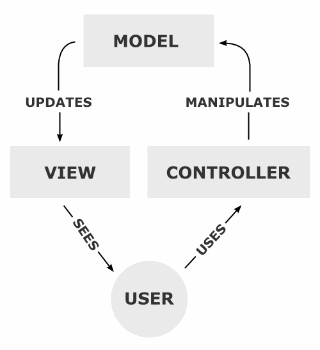
\includegraphics[scale=0.5]{imagenes/MVC-Process.png} 
	\caption{ Diagrama del patrón Modelo Vista Controlador, imagen de \url{https://es.m.wikipedia.org/wiki/Archivo:MVC-Process.png} } \label{fig:MVC-Process.png}
\end{figure}

El controlador recoge las entradas de usuario y las gestiona, en nuestro caso recogerá las pulsaciones del teclado y el movimiento del ratón que se transformarán en el movimiento de la cámara por ejemplo. El controlador será el que contenga todo el tema del procesado geométrico, el modelo contendrá las estructuras de datos para alojar los vértices, caras, semi-aristas aladas, etc. \\

\newpage
\section{ Diagrama de clases}
El diagrama de clase nos permite ver cómo se van a estructurar las clases de manera general además de ver la interacción entre ellas. El diagrama de clases se ve en la figura \ref{fig:diagramaClases.png}

\begin{figure} %con el [H] le obligamos a situar aquí la figura
	\centering
	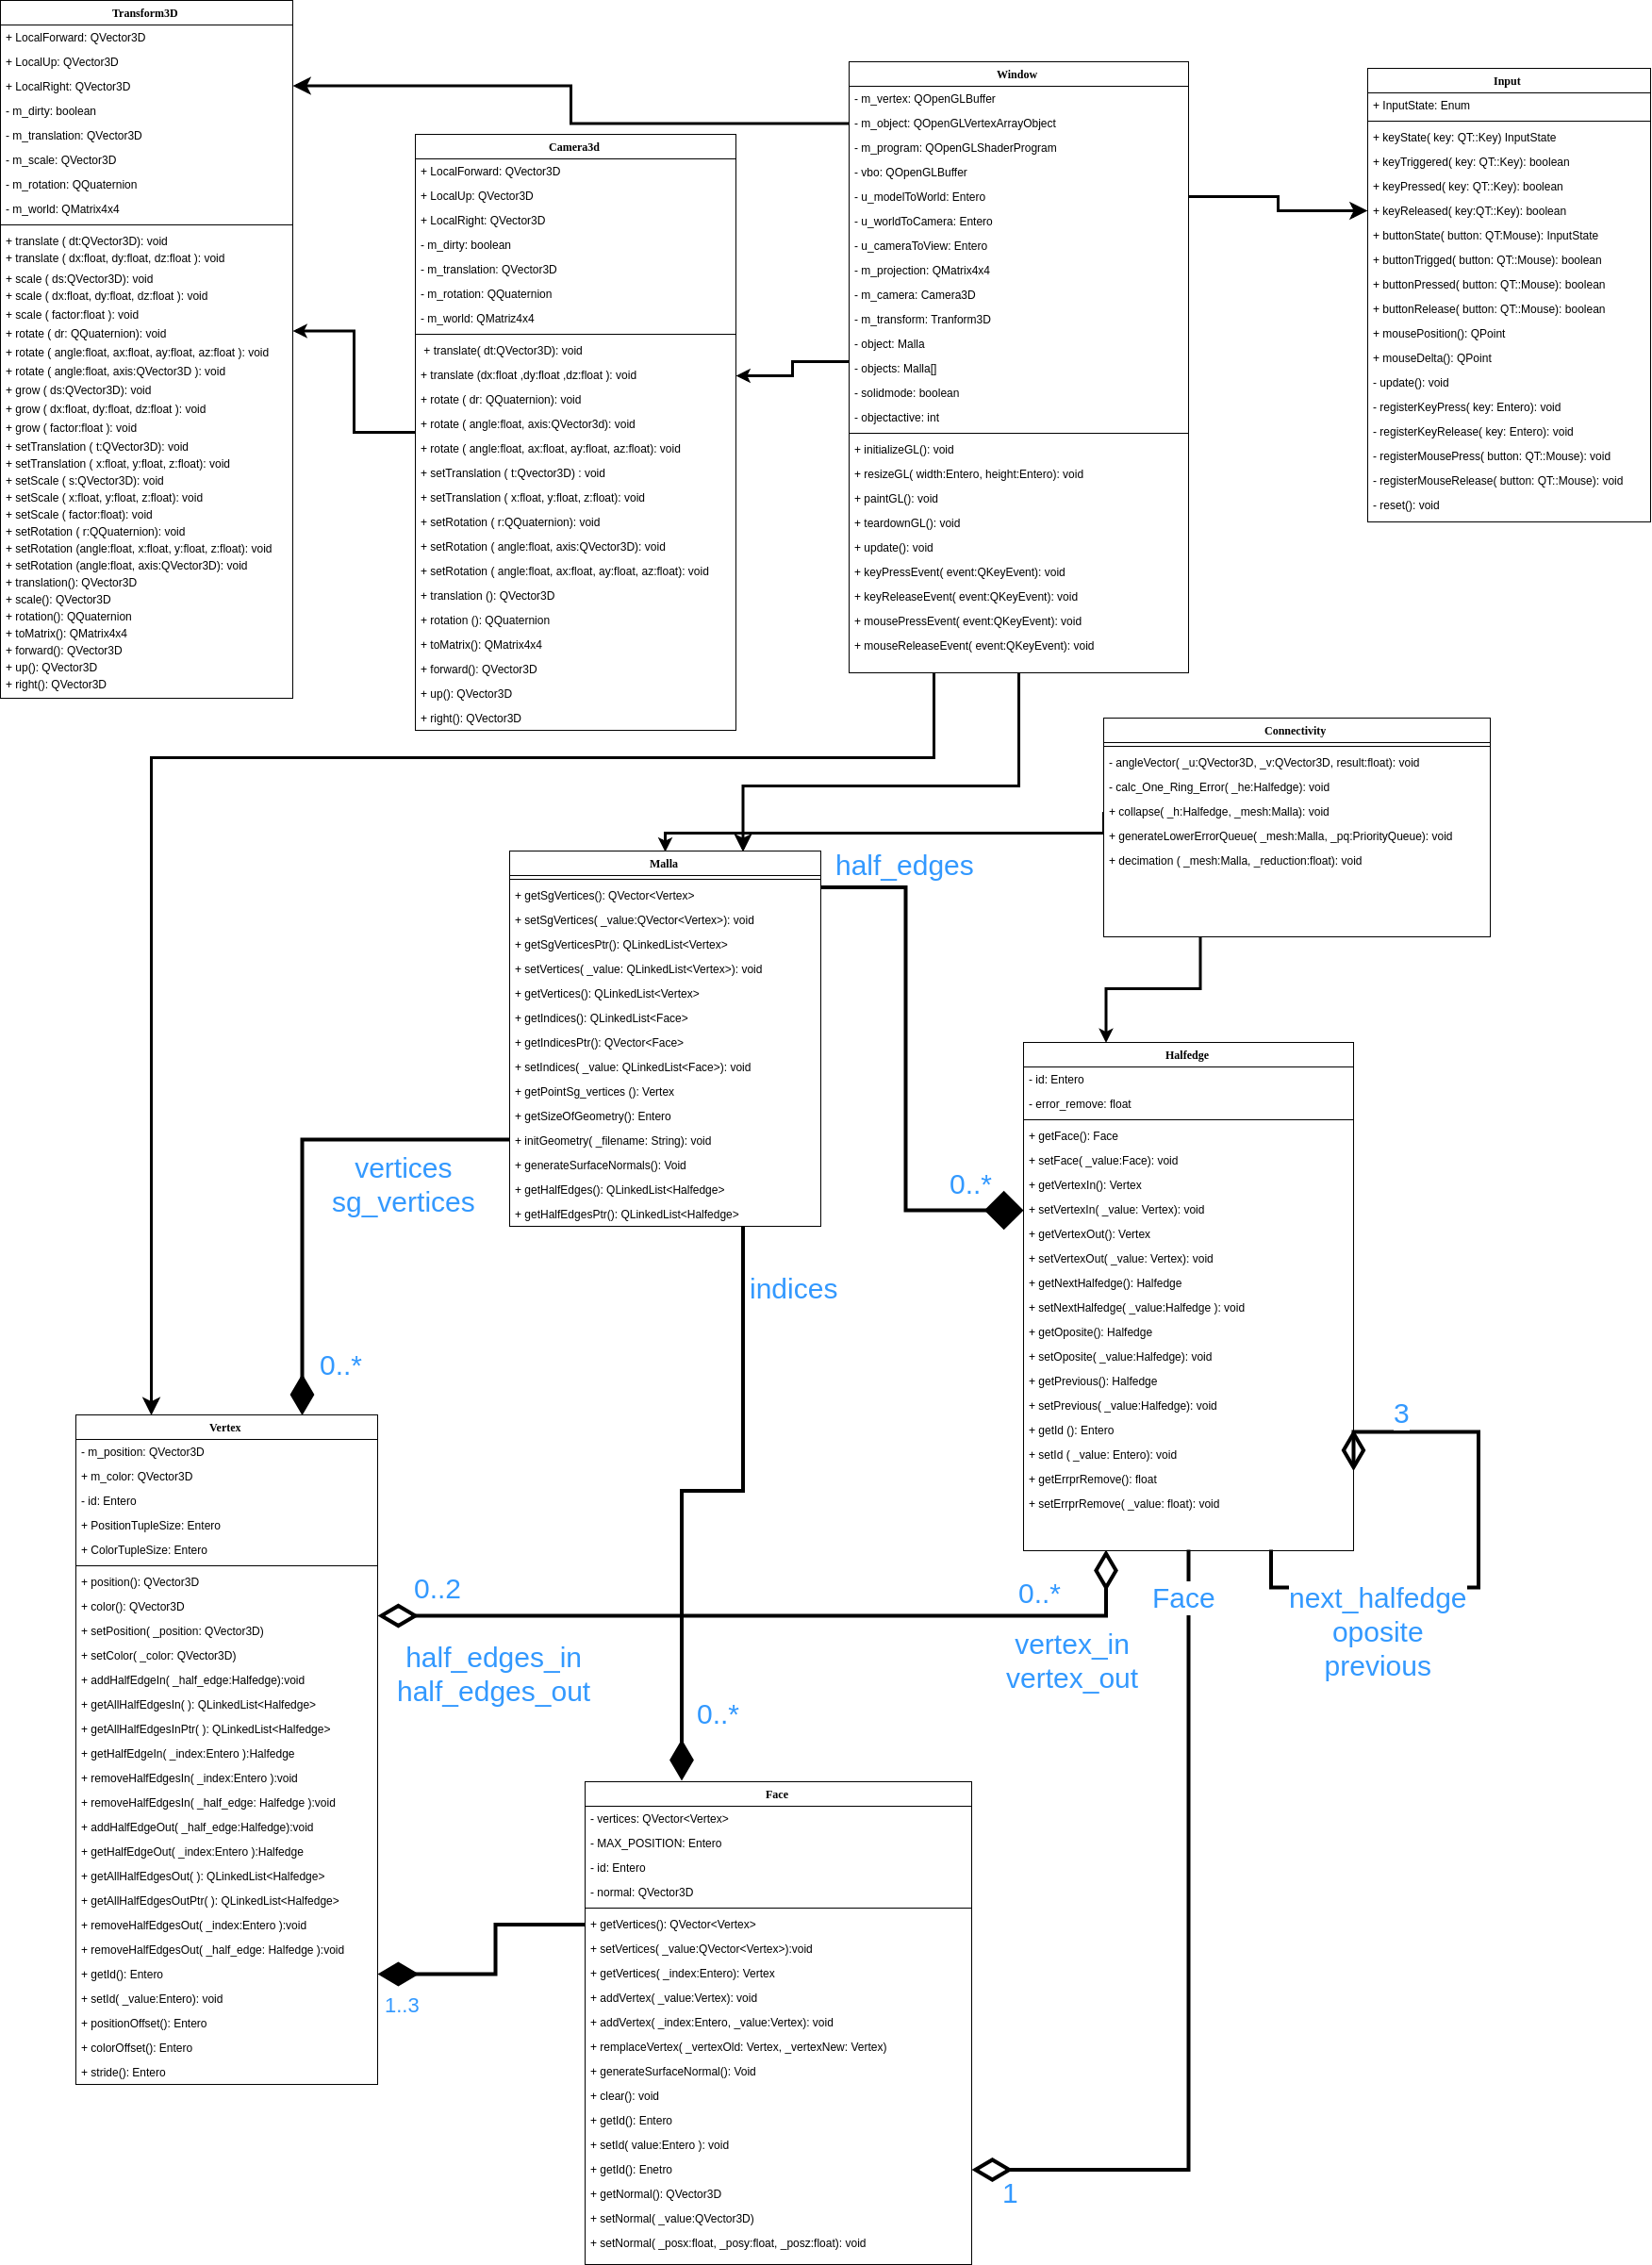
\includegraphics[scale=0.25]{imagenes/diagramaClases.png} 
	\caption{ Diagrama de clases } \label{fig:diagramaClases.png}
\end{figure}

